\chapter{Optimizing the variational bound stochastically}
\label{chapter:stochastic_variational_optimization}

Estimating an arbitrary probability distribution $p(x)$ is a
fundamental problem in statistical modeling.  This problem arises in
posterior inference, for example, where we seek to estimate a
conditional $p(x | y)$ of latent variables $x$ given observations $y$.
There are two main classes of solutions---Markov chain Monte Carlo
(MCMC)~\cite{bishop:2006} and variational methods~\cite{jordan:1999}.
In MCMC, we define a Markov chain whose stationary distribution is the
target distribution.  We run the chain to try to collect independent
samples from the stationary distribution, and then use them to form an
approximation.  In variational inference, we posit a parameterized
family of distributions $q_\theta(x)$ and find the member of that
family that is ``closest'' to the true posterior.  This turns the
problem of inference into one of optimization.

Deriving and implementing a variational inference algorithm can be
painstaking.  It involves defining the variational family, forming an
objective function, taking derivatives with respect to the variational
parameters, and running an optimization algorithm.  In this paper, we
present an alternative algorithm for variational inference.  Our
algorithm circumvents many of the challenges to using variational
inference by optimizing the variational objective function
stochastically.

To do this, we form the derivative of the variational objective as an
expectation with respect to the variational distribution. We then
sample from that distribution to obtain realizations of a stochastic
gradient.  Our algorithm is a ``black box'' algorithm in that it only
requires that we evaluate the joint likelihood $p(x, y)$ of the hidden
and observed variables (up to a constant factor), the variational
likelihood $q(x)$ (up to a constant factor), and the derivative of
$\log q(x)$.  (Note that this derivative can be reused across
variational inference problems.)  Unlike other automated approaches to
variational inference \cite{winn:2004}, we have no other restrictions
on the model or variational family, e.g., that the hidden variables
come in conjugate pairs or that the variational distributions are in
the exponential family.

% dmb: above, cite something like the vibes jmlr paper

% dmb: i also think that this detail (below) can go in the quasi-MC
% section.

% First, we demonstrate that quasi-Monte Carlo sampling (discussed in
% Section~\ref{section:minibatch_sampling}) lets us fit variational
% posteriors more efficiently.

% dmb: issues with the description of carbonetto, 1 unbiased estimate?
% 2 the true posterior is not in the exponential family

There have been several recent algorithms that are similar in spirit
to ours.  Both Carbonetto et al. and Graves perform variational
inference by taking samples from the variational posterior to estimate
a gradient \cite{carbonetto:2009, graves:2011}.  Carbonetto et
al. assume that the variational distribution comes from the
exponential family \cite{carbonetto:2009}.  Graves \cite{graves:2011}
approximates the first-order gradient for fitting a neural network.

% dmb: for publication, let's remove "significantly".  for the
% submission, it sounded right.

% dmb: below, let's consider putting the restrictions later in the
% paper and just refering to the section.  then we can add the few
% sentences below to the previous paragraph.

Our work significantly expands on this research.  We make weaker
assumptions than Carbonetto et al. \cite{carbonetto:2009} on the forms
of $p$ and $q_\theta(x)$.  Our posterior $p(x | y)$ and $q(x)$ must be
well-behaved---the KL-divergence between $p(x | y)$ and $q(x)$ must
exist, $\log q_\theta(x)$ must be differentiable almost everywhere,
and $q_\theta$ must have finite variance---but is otherwise
unrestricted.  Our method can be used for a wider variety of
statistical models, with benefits over both MCMC and traditional
variational inference.

% dmb: below, add this point to the experiments.  (and, maybe, the abstract.)

% We have also provided a library to allow other researchers to perform
% inference with several variational posteriors.


%%% Local Variables: 
%%% mode: latex
%%% TeX-master: "nips2012"
%%% End: 

\section{Stochastic optimization of the variational objective}

We begin this section by reviewing variational inference for
approximating posterior distributions.  We then derive our algorithm
for optimizing the variational objective with stochastic optimization.
We discuss an illustrative example and describe several extensions to
the algorithm.

\subsection{Variational inference}

Variational methods are a fast, deterministic alternative to MCMC for
approximate inference \cite{jordan:2003,jordan:1999}. Variational
methods posit a parameterized family of distributions $q_{\theta}(x)$
and try to find the member (i.e., the setting of variational
parameters $\theta$) that is closest in KL-divergence to the posterior
$p(x | y)$,
\begin{align}
  \arg \min_{\theta} \mbox{KL}(q_\theta || p) = \arg \min_{\theta}
  \int q_\theta(x) \log \frac{q_\theta(x)}{p(x | y)} dx.
  \label{equation:stochastic_variational_objective}
\end{align}
We select the family to make this optimization problem tractable.  A
commonly chosen family is the mean-field family, where the variational
distribution is fully factorized.  For example, if $x$ is a collection
of real-values that are dependent in $p(x | y)$ then the mean-field
distribution might be a product $\prod_K \mathcal{N}(\mu_k,
\sigma_k^2)$ of independent Gaussian distributions.

% dmb: i wasn't clear about how we select a family to capture
% statistics of interest.  it sort of makes sense, but not in a
% concrete way.

% to capture statistics of interest, such as marginal means, and

% . Often this family consists of only fully factorized
%distributions; such an assumption is known as \emph{naive mean-field
%  variational inference}.

Optimizing \myeq{stochastic_variational_objective} is equivalent to optimizing
the ``evidence lower bound'' (ELBO) $\mathcal{L}_\theta$:
\begin{eqnarray}
  \log p(y) \ge \expectq{\log p(x, y) - \log q_\theta(x)}
  =: \mathcal{L}_\theta,
  \label{equation:stochastic_traditional_variational_objective}
\end{eqnarray}
where the slack of the bound is equal to the KL divergence from
\myeq{stochastic_variational_objective}.  Typical variational inference
algorithms optimize this bound by coordinate ascent.  This requires
evaluating $\expectq{ \log p(x, y) - \log q_\theta(x)}$ and its
gradient with respect to $\theta$. If the variational distribution is
not conjugate to the joint distribution $p(x, y)$, the expectation
$\expectq{ \log p(x, y)}$ will not be analytically tractable. We may
then need to perform further bounds or approximations
\cite{jaakkola:2000,jordan:1999,bickel:2007,braun:2007}.


%%  A Gaussian variational
%% marginal distribution might represent a real-valued random variable,
%% and a Dirichlet distribution might represent a multinomial random
%% variable \cite{bishop:2006}.

% dmb: below, i don't think the first point is too strong, but i don't
% think anyone will dispute it either.

This procedure makes variational methods challenging for two reasons.
First, they require a steep learning curve and careful attention to
detail to derive the coordinate updates. Second, this process must be
repeated each time the model $p(x, y)$ changes form.  Deriving the
variational algorithm becomes a bottleneck when we seek rapid model
development.

%% These simplifying assumptions -- an approximate, fully factorized
%% posterior with further simplifying bounds -- make it possible to
%% express the lower bound in terms of the variational parameters
%% $\theta$.  This is followed by coordinate or gradient ascent.

%% More complicated variational posteriors are rarely considered because
%% the expansion $\expectq{ \log p(x, y) - \log q_\theta(x)}$ may have no
%% closed form, or it may be be hard to bound.  As we show later, we can consider a
%% wider variety of variational posteriors when algebraic approximation
%% is not a bottleneck.

%%% Local Variables: 
%%% mode: latex
%%% TeX-master: "nips2012"
%%% End: 

%% We will avoid requiring the symbolic expansion of $\expectq{\log
%% p(x, y)}$, which is typically required for variational inference.

\subsection{Stochastic optimization of the variational objective}

We now describe an alternative method for optimizing the ELBO
$\mathcal{L}$. We form a noisy estimate of the gradient using
Monte-Carlo integration \cite{graves:2011,wei:1990,carbonetto:2009},
and follow it with stochastic optimization~\cite{robbins:1951}.  This
avoids difficult derivations; we need only evaluate $\log p(x, y)$,
$q_\theta(x)$, and $\nabla \log q_\theta(x)$.

% \subsubsection{Stochastic optimization.}
% Stochastic optimization is used to optimize an objective function with
% a stochastic approximation of the gradient.  The objective typically
% takes the form $\mathbb{E}_{\mathcal{D}} \left[ \sum_{N} f(x_n,
% \theta) \right]$, where the expectation is taken over the
% data-generating distribution $\mathcal{D}$.
% \cite{robbins:1951,bottou:2004}. In the simplest case, $\theta$ is
% optimized sequentially by using a gradient of the objective for each
% \emph{iid} training example $x_1, \ldots, x_N \sim \mathcal{D}$:
% \begin{align}
%   \label{equation:stochastic_optimization}
%   \theta_n \gets \theta_{n-1} + \frac{\eta}{n^k} \partl{f(x_n, \theta)}{\theta} \Bigr|_{\theta_{n-1}},
% \end{align}
% \paragraph{Stochastic optimization applied to our method}
%As with stochastic optimization, we follow a stochastic gradient
%$\partlapprox{\mathcal{L}_\theta}{\theta}$ of our objective.  To this

We now show that the gradient of
\myeq{equation:stochastic_traditional_variational_objective} can be written as an
expectation.  We first exchange integration and
differentiation\footnote{This assumes the support of $q_\theta$ is not
  a function of $\theta$, and that $\log q_\theta(x)$ and $\nabla \log
  q_\theta(x)$ are continuous with respect to $\theta$.}, and apply
the chain the rule,
\begin{align}
 \nabla \mathcal{L}_\theta &= \nabla \Bigl[
  \int q_{\theta}(x) (\log p(x, y) - \log q_{\theta}(x))
  dx \Bigr] \\ \nonumber
  & = \int \nabla \Bigl[ q_{\theta}(x) (\log p(x, y) - \log
     q_{\theta}(x)) \Bigr] dx  \\ \nonumber
     &= \int \nabla q_{\theta}(x) (
     \log p(x, y) - \log q_{\theta}(x) - 1) dx.
\end{align}
We can write this as an expectation by using the identity
$q_\theta(x) \nabla \log q_\theta(x) = \nabla q_\theta(x)$,
\begin{align}
  \label{equation:gradient-as-expectation}
  \nabla \mathcal{L}_\theta =
  \expectq{\nabla \log q_\theta(x) \left(\log p(x,y) - \log
      q_{\theta}(x) - 1 \right)}
\end{align}
Now we use Monte Carlo integration to form an unbiased estimate of the
gradient at $\theta = \theta_0$.  We obtain $M$ samples from the
variational distribution $q_{\theta_0}(x)$, $\{x_{1}, \ldots, x_{M}\}$
and approximate,
\begin{align}
  \label{equation:svo_gradient}
  \nabla \mathcal{L}_\theta \approx \frac{1}{M} \sum_{m=1}^M
  \nabla \log q_{\theta}(x_{m}) \Bigr|_{\theta_0}
  (\log p(x_{m} , y) - \log q_{\theta_0}(x_{m}) - C).
\end{align}
Note we replaced the one in \myeq{gradient-as-expectation} with a
constant $C$.  This follows because $\expectq{\nabla \log q_\theta(x)}
= 0$.  For now we will assume $C$ equals zero, but see
\mysec{setting-c} for how to improve performance by adjusting this
constant.

Related estimates of similar gradients have been studied in
recent work~\cite{carbonetto:2009,graves:2011} and in the context of
expectation maximization~\cite{wei:1990}.

The quality of this estimate depends on the sample size $M$.  A small
number of samples leads to a fast but crude approximation, while a
large number of samples will be slower but more accurate.  We will
explain in Section~\ref{section:minibatch_sampling} how to decrease
the variance of this approximation by using batches of carefully
selected, non-\emph{iid} samples and provide an experiment to explore
the effect of sample size.


% dmb: above, get to the bottom of the difference between earl

% dmb: write a section about C in the extensions part.

% !!! i am here: the next step is to talk about stochastic
% optimization and convergence.  then discuss the advantages of this
% algorithm (at the end).  [i.e., reorganize this section]  option:
% turn the gaussian example into a \paragraph.  also, in discussing
% convergence is where we differentiate to the usual use of stoch opt
% and, in particular, hoffman's paper.

With regard to the model, the gradient estimate in \myeq{svo_gradient}
only requires we can evaluate the joint distribution.  This means that
variational inference can take the form of a ``black box'': we do not
need to compute expectations of $p(x, y)$ or gradients of
$\mathcal{L}_\theta$ with respect to $q_\theta$ or $\theta$.  The
other requirements---that we can sample from the variational
distribution $q_\theta(x)$ and evaluate its log and gradient of its
log---are usually easy.  (And, if not, they can be worked out once and
then placed in reference for use in many variational algorithms.)  We
give concrete examples of the gradient of the log for several types of
distributions in \mysec{gaussian}, \mysec{complicated_posteriors} and
in the supplementary materials.
%\ref{section:dirichlet_multinomial},

% dmb: above, give the specific sections of the supplement and use \S
% S.1.


\textbf{Stochastic optimization.}  We can now embed this approximation
in a stochastic optimization algorithm.  In this algorithm, we proceed
with a sequence of estimates $q_{\theta_0}, q_{\theta_1}, \ldots$ of
the variational distribution. On the $n$th iteration, we use
Monte-Carlo samples from the previous distribution $q_{\theta_{n-1}}$
to stochastically estimate the gradient to find the next
distribution:
\begin{align}
  \label{equation:svo_update}
  \theta_n \gets & \theta_{n-1} +
  \frac{\eta}{n^k} \partlapprox{\mathcal{L}_\theta }{ \theta } \Bigr|_{\theta_{n-1}},
\end{align}
where $\eta > 0$ is a learning rate parameter and $k \in (0.5, 1.0]$
  \cite{carbonetto:2009}. Importantly, the expectation of the
  stochastic gradient, $\expectd{\partl{f(x_n, \theta)}{\theta}}$, is
  the gradient of the objective (up to a constant factor).
% Multiple samples $x_1, \ldots, x_M$ are sometimes combined in a
% \emph{minibatch} for a better estimate $\sum_M \partl{f(x_m,
%   \theta)}{\theta}$ of the gradient.
We call this method first-order Stochastic Variational Optimization
(SVO) and summarize it in Algorithm 1. % ~\ref{figure:first_order_algorithm}.

\textbf{Convergence.} We apply these updates until a predefined
convergence criterion is met (we give details in the next section).
In most stochastic optimization settings, the sampling distribution
$\mathcal{D}$ is stationary, and many theoretical results demonstrate
when and how stochastic optimization converges to an optimum of the
objective with this assumption \cite{bottou:2004,robbins:1951}.  We
violate this assumption because the distribution $q_\theta$ changes in
each iteration.  Still, we find that this method reliably converges in
practice.

\subsubsection{Example: Gaussian variational marginal}
\label{section:gaussian}
In the next section we will describe ways to improve this gradient
ascent algorithm (Equation~\ref{equation:svo_update}), but first we
illustrate this method by estimating an ``unknown'' posterior with a
Gaussian variational posterior.

We let $p(x, y)$ be the joint likelihood. In this example, $p(x, y)$
is a synthetic distribution: a unimodal mixture of two Gaussians,
$\mathcal{N}(x | 5.1, 12)$ (with component weight 0.5) and
$\mathcal{N}(x | 5, 3)$ (with component weight 1).  We illustrate this
distribution in
Figure~\ref{figure:univariate_comparison_approximation}.  We will make
only the joint likelihood $\log p(x, y)$ of this posterior available
to SVO (note that $y$ is a dummy variable in this example).
\begin{figure}[t!]
  \center
  \vspace{-32pt}
  \includegraphics[width=0.45\textwidth,height=0.21\textheight]{chapter_stochastic_variational_optimization/figures/laplace_approximation.pdf} \\
  \vspace{-20pt}
  \caption{A non-conjugate posterior density (dashed) and a Gaussian
  variational approximation (solid).}
  \label{figure:univariate_comparison_approximation}
\end{figure}

We initialize the Gaussian variational posterior to the distribution
$q_{\mu_1, \sigma_1^2}(x) = \mathcal{N}(x | \mu_{1}, \sigma_{1}^2)$,
with $\mu_1=0$ and $\sigma_1^2=4$. We proceed by drawing samples $x_1,
\ldots, x_{15} \sim N(x | \mu_1, \sigma_1^2)$ and calculating, for each
sample, the gradients
\begin{align}
  \label{equation:gaussian_mean_gradient}
  \partl{\log q_{\mu, \sigma_1^2}(x_m)}{\mu} \Bigr|_{\mu_{n1}}
  = \partl{}{\mu} \frac{-(x_m - \mu)^2}{2 \sigma_1^2} \Bigr|_{\mu_{1}}
  = \frac{x_m - \mu_1}{\sigma_1^2},
\end{align}
using the Gaussian density $q_{\mu_1, \sigma_1^2}$.  We
estimate a gradient of the objective by combining these samples
(Equation~\ref{equation:svo_gradient})
\begin{align}
  \partlapprox{\mathcal{L}_{\mu, \sigma_1^2}}{\mu} \Bigr|_{\mu_{1}} &
  %    & \hspace{-65pt}
  \hspace{-5pt} = \hspace{-2pt} \frac{1}{M} \sum_M \hspace{-1pt}\frac{x_m\hspace{-1pt}-\mu_1}{\sigma^2_1}
  \hspace{-2pt} \left( \log p(x_m, y)-\hspace{-1pt} \log q_{\mu_1, \sigma_2^2}(x_m) \right) \\ \nonumber
%  & \approx \frac{1}{M} \sum_M \frac{x_m - \mu_1}{\sigma^2_1}
%    \log p(x_m, y). \\ \nonumber
%  \vspace{-20pt}
\end{align}
%where we make the final (optional) approximation by taking advantage
%of the symmetry of the Gaussian $q$: $\expectq{\partl{}{\mu} \log
%q_{\mu, \nu}(x) \times \log q_{\mu, \nu}(x)} = 0$.

\begin{figure}[t]
  \center
  \vspace{-10pt}
  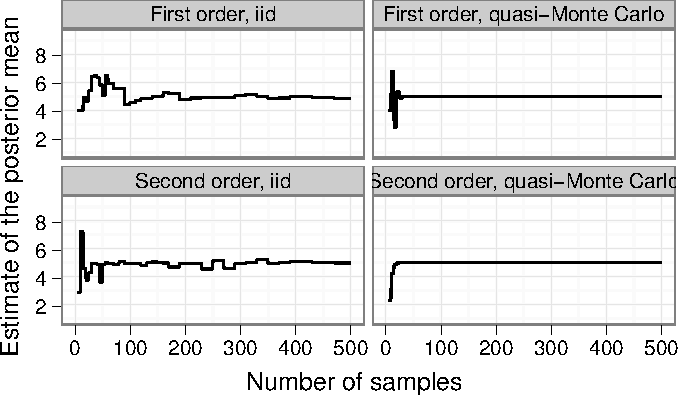
\includegraphics[width=0.65\textwidth]{chapter_stochastic_variational_optimization/figures/mean_estimate_by_order_sampling.pdf} \\
  \vspace{-10pt}
  \caption{A comparison of our algorithm using first-order
  vs. second-order updates (top vs. bottom); and estimating gradients
  using \emph{iid} samples from $q$ vs. quasi-Monte Carlo samples from
  $q$ (left vs. right).}
  \label{figure:comparision_order_sampling}
  \vspace{-15pt}
\end{figure}
and finally update the mean $\mu$ (Equation~\ref{equation:svo_update}):
\begin{align}
  \label{equation:gaussian_mean}
  \mu_2 \gets \mu_{1}
    + \frac{\eta_\mu}{1^k}
    \partlapprox{ \mathcal{L}_{\mu, \sigma_1^2} }{\mu} \Bigr|_{\mu_{1}}.
\end{align}
The update for variance is similar, but we optimize $\nu = \log
\sigma^2$ instead of $\sigma^2$:\footnote{$\sigma^2$ must be strictly
positive, so $\nu$ is a more natural choice for stochastic updates).}
\begin{align}
  \label{equation:gaussian_variance_gradient}
%  \partl{\log q_{\mu, \nu_1}(x)}{\nu} \Bigr|_{\nu_{1}}
%  & = \frac{ (x_{m} - \mu_{1})^2 }{ \exp(\nu_{1}) } - 1 \\ \nonumber
  \partlapprox{ \mathcal{L}_{\mu_1, \nu} }{\nu} \Bigr|_{\nu_{1}} & \approx
  \frac{1}{M} \sum_{m=1}^M \bigg[ \left( \frac{ (x_{m} - \mu_{1})^2 }{ \exp(\nu_{1}) } - 1 \right) \\ \nonumber
  & \hspace{-30pt} \times \left( \log p(x_m, y) - \log q_{\mu_1, \nu_1}(x_m) \right) \bigg]. \\ \nonumber
\end{align}
The variance is then updated with Equation~\ref{equation:svo_update}:
$ \nu_2~\gets \nu_{1} + \frac{\eta_\nu}{1^k} \partlapprox{ \mathcal{L}_{\mu_1, \nu} }{\nu} \bigr|_{\nu_{1}}$ .


\paragraph{Testing convergence.}
We repeated this process for iterations $n = 1, 2, \ldots$ until
convergence.  The variational estimate of the mean by the total number of
samples is shown in Figure~\ref{figure:comparision_order_sampling}
(top-left corner).  To test convergence, we estimated the evidence
lower bound at each iteration,
\[
  \mathcal{L}_n = \frac{1}{M} \sum_M \left( \log p(x_{nm}, y) - \log
q_{\theta_n}(x_{nm}) \right).
\]
We performed these updates until the exponential moving average
$\Delta_{\mbox{est},n} \gets 0.8 \Delta_{\mbox{est},{n-1}} + 0.2
(\mathcal{L}_n - \mathcal{L}_{n-1})$ of the ELBO dropped below one.
Any time this happened, we scaled the number $M$ of samples by a
factor of 1.2. When the moving average dropped below one and $M >
500$, we stopped the algorithm.

Note that the functional form of $p(x, y)$ was never used in these
updates: only the form of $q(x)$ was used.  A variety of other
variational posteriors are used in practice.  We provide these
gradients for Dirichlet and multinomial posteriors, which are
conjugate to multinomial and indicator random variables respectively,
in the supplementary materials. To fit these variational
distributions, we need to compute $\partl{\log q_\theta}{\theta}$ as
in Equations~\ref{equation:gaussian_mean_gradient}
and~\ref{equation:gaussian_variance_gradient}; the other steps are
mechanical.

\subsection{Improving performance}

The algorithm described above lays the foundation for our approach.  We
now make several adjustments to complete the algorithm.  These
adjustments revolve around (1) improving samples used to estimate the
gradient, which we can do because we have intimate knowledge of
$q_{\theta_n}$, and (2) improving step sizes with second-order updates.

\subsubsection{Minibatch sampling}
\label{section:minibatch_sampling}
The stochastic gradients in Equation~\ref{equation:svo_gradient} were
estimated with ``minibatches'' of $M$ \emph{iid} samples from $q$.  As
Figure~\ref{figure:comparision_order_sampling} (top left) shows, the
first-order estimate may need many samples to reach satisfactory
convergence, a common observation in stochastic optimization.

One key insight for our algorithm is that we have more control over
samples because we have perfect knowledge of $q_\theta$.  This
contrasts with many stochastic optimization methods, in which samples
may be drawn \emph{iid} from an unknown distribution $\mathcal{D}$.
By carefully selecting minibatches with non-\emph{iid} samples, we can
decrease the variance of our estimate of the ELBO $\partl{ \mathcal{L}_\theta
}{\theta}$.  Quasi-Monte Carlo methods such as the Latin hypercube
design have been developed for exactly this purpose
\cite{tang:1993,owen:1998,niederreiter:1992}.

To sample values from a univariate variational distribution $q$, we
select $M$ equidistant points from the uniform distribution and pass
these points through the inverse CDF of $q$.\footnote{For a truly
  unbiased minibatch sample from $q$, these points could be jittered
  with uniform noise within each interval.} To sample from
multivariate distributions $\Pi_D q_d$, we select $M$ samples from
each of the $D$ distributions, randomly permute samples from each
distribution, and group them into $M$ $D$-variate samples. We increase
the number of samples as the algorithm converges as described in the
experiments section
\cite{wei:1990}. Figure~\ref{figure:comparision_order_sampling} (top
right) illustrates the effect of quasi-Monte Carlo sampling on
convergence of SVO.

Numerical estimates with these samples can be vectorized, which can
speed up computation significantly.\footnote{Vectorization uses
  software libraries such as BLAS and hardware such as GPUs to use
  samples more efficiently.}  This use of samples contrasts with
standard MCMC methods, which require sequential, dependent samples
from a given random variable.  When MCMC does not require sequential
samples (e.g., updates to variables which are conditionally
independent), SVO does not require sequential samples.

 \subsubsection{Second-order updates}
 \label{section:second_order_updates}
\begin{figure}
%   \begin{algorithm}[tb]
     \begin{algorithmic}[1]
    \setlength{\topsep}{1pt}
    \setlength{\itemsep}{2pt}
    \setlength{\parskip}{1pt}
    \setlength{\parsep}{1pt}

     \STATE $n \gets 1$
    \WHILE{not converged}
    \STATE Draw samples $x_{n1}, \ldots, x_{nM} \sim q_{\theta_{n - 1}}$ using quasi-Monte Carlo sampling.
    \STATE Compute $\partl{\log q_{\theta_n}(x_{nm})}{\theta} \Bigr|_{\theta_{n-1}}$ and
    $\partll{\log q_{\theta_n}(x_{nm})}{\theta} \Bigr|_{\theta_{n-1}}$. % for $m = 1 \ldots, M$.
    \STATE Estimate $\partl{\mathcal{L}_\theta }{\theta} \Bigr|_{\theta_{n-1}}$ using Equation~\ref{equation:svo_gradient}.
    \STATE Estimate $\partll{\mathcal{L}_\theta }{\theta} \Bigr|_{\theta_{n-1}}$ using Equation~\ref{equation:empirical_second_order_estimates}.
    \STATE Update $\theta$, using Equation \ref{equation:second_order_updates}:
        \vspace{-10pt}
	\begin{align*}
     	   \displaystyle \theta_n \gets \theta_{n-1} - \left( 
     	\partll{\mathcal{L}_\theta }{\theta}
     	\right)^{-1}
     	\partl{\mathcal{L}_\theta }{\theta}.  \end{align*}
    \vspace{-15pt}
    \STATE $n \gets n + 1$ % (until convergence)
    \ENDWHILE
   \end{algorithmic}
     \caption{Second-order SVO. We begin with a variational distribution
       $q_{\theta_0}(x)$ and joint likelihood $p(x, y)$.  }
     \label{figure:second_order_algorithm}
\end{figure}
%   \end{algorithm}

We also note that the step size parameters $\eta$ and $k$ have a large
impact on convergence to an optimal solution: they must be carefully
tuned in both stochastic optimization and our algorithm. We circumvent
the challenge of selecting step size with second-order updates, which
are sometimes used in stochastic optimization
\cite{robbins:1951,bottou:2004} and were used by
\citet{carbonetto:2009} and \citet{wei:1990}.  To derive the
second-order updates, we make a Taylor approximation of the
variational objective $\mathcal{L}_\theta$
(Equation~\ref{equation:stochastic_traditional_variational_objective}) around the
current estimate $\theta_0$:
\begin{align}
  \mathcal{L}_\theta \approx & \mathcal{L}_{\theta_0} + ( \partl{\mathcal{L}_\theta }{\theta} \Bigr|_{\theta_0} )^T \Delta_\theta
 + \Delta_\theta^T ( \frac{\delta^2 \mathcal{L}_\theta }{\delta \theta \delta \theta^T} \Bigr|_{\theta_0} ) \Delta_\theta, \\ \nonumber
\end{align}
where $\Delta_\theta = \theta - \theta_0$.  This approximation becomes
exact as $\theta_0$ approaches the optimal solution.

In addition to estimating the gradient $\partl{\mathcal{L}_\theta }{\theta} \Bigr|_{\theta_0}$, we also estimate the curvature
$\partll{\mathcal{L}_\theta }{\theta} \Bigr|_{\theta_0}$
empirically with samples:
\begin{align}
  \label{equation:empirical_second_order_estimates}
  \displaystyle \partll{\mathcal{L}_\theta }{\theta} & \approx
  \frac{1}{M} \sum_M \Bigg(
  \left( \partl{\log q_\theta(x_{nm})}{\theta} \Bigr|_{\theta_0} \right)^2 \\ \nonumber
  & \hspace{35pt} \times \left( \log p(x_{nm},  y) - \log q_{\theta_0}(x_{nm}) - 1 \right)  \\ \nonumber
 &   \hspace{-25pt} + \left( \partll{\log q_\theta(x_{nm})}{\theta} \Bigr|_{\theta_0} \right) \left( \log p(x_{nm},  y) - \log q_{\theta_0}(x_{nm}) \right) \Bigg). \\ \nonumber
\end{align}
The estimate of the optimum is then
\begin{align}
  \displaystyle \theta \gets \theta_0 - \left( 
  \partll{\mathcal{L}_\theta }{\theta} \Bigr|_{\theta_0}
  \right)^{-1}
  \partl{\mathcal{L}_\theta }{\theta} \Bigr|_{\theta_0}.
  \label{equation:second_order_updates}
\end{align}
This algorithm is summarized in
Figure~\ref{figure:second_order_algorithm}, and it can be used instead
of the first-order algorithm
(Figure~\ref{figure:first_order_algorithm}), just as in stochastic
optimization \cite{bottou:2004}.  The results of applying this
algorithm to the synthetic dataset described in the last section is
shown in Figure~\ref{figure:comparision_order_sampling} (bottom two
panels).  Second order methods can help to avoid both high variance in
a posterior estimate and poor learning rates.

We can approximate both the gradient and curvature arbitrarily well by
increasing the number of samples $M$, provided that $q$ and $p$ are
well-behaved.  This turns the problem into approximate Newton-Raphson
optimization, which means that this approach can converge more
reliably than stochastic optimization by using more (and better)
samples during the final updates.  It also means that a tunable
learning rate is no longer necessary.

\subsection{Multivariate distributions}
Most interesting latent-variable models are multivariate, so we now describe
our algorithm in the multivariate setting.  With traditional variational
inference, we update the posterior estimate $q_\theta$ of each hidden
random variable $x_i$ successively, given the current estimate of the
remaining variables' distributions.  This update is typically
accomplished by gradient or coordinate ascent.  In these cases, the
distributions of hidden random variables are usually represented by
their expectation under the variational distribution.

SVO optimizes the objective similarly: the distribution of each hidden
random variable $x_i$ is updated by holding the distributions of the
remaining hidden variables fixed.  To represent the distributions of
variables in $x_i$'s Markov blanket, SVO uses samples from their
variational posteriors.

\subsection{Related work}

\paragraph{Stochastic optimization.}
SVO differs from traditional stochastic optimization in several
important ways.  We draw a contrast from methods which optimize a
variational lower bound with \emph{iid} training examples
\cite{hoffman:2010} from an unknown distribution; we optimize the
probability distribution with respect to which we are taking an
expectation.  Further, the samples we use to optimize this bound are
drawn from this distribution.  This is not the case for stochastic
optimization in general.
%which is known to us.
% Although we are able to control samples much better than we could with
% vanilla stochastic optimization, this does not mean that our method is
% an alternative or competitor to stochastic optimization.
We address a specific problem using ideas from stochastic
optimization, making improvements for the specific problem at hand.
Many of these improvements do not apply in the general stochastic
optimization setting.

\paragraph{Stochastic sampling with variational inference.}
\citet{carbonetto:2009} used stochastic optimization in an approach
conceptually very similar to ours.  They sample from the variational
posterior and use importance sampling along with second-order updates
to estimate a similar gradient.  They further
assume that the family of variational distributions includes an
unbiased estimate of the true posterior, and that both the variational
posterior and true posterior come from the same exponential family.

We make weaker assumptions on the forms of $p$ and $q_\theta(x)$. Our
posterior $p(x | y)$ and $q(x)$ must be well-behaved: the
KL-divergence between $p(x | y)$ and $q(x)$ must exist, and it must be
approximable with Monte-Carlo methods.  We further require that (1)
$\log q_\theta(x)$ be differentiable almost everywhere and (2)
$q_\theta$ have finite variance.

\citet{carbonetto:2009} used importance sampling to approximate a
gradient and require learning rates to be carefully set.  We address
both of these by using the sampling methods discussed in
Section~\ref{section:minibatch_sampling}.

\citet{wei:1990} use Monte-Carlo sampling to perform the E-step of EM
using a finite-sum approximation of an integral. While they
explicitly outline the gradient and Hessian of the expectation, they
never use these values.
%   We note that the methods discussed in
% Section~\ref{section:minibatch_sampling} -- namely, careful sampling
% methods -- make this method more robust to noise
% \cite{tang:1993,owen:1998,niederreiter:1992}.

% \paragraph{Samples for }
% The true and variational posteriors $p(x_i, x_{\i} | y), q(x_i,
% x_{\i})$ are both proportional to $p(x_i | x_{\i}, y), q(x_i |
% x_{\i})$.

\section{Empirical study}

In this section we studied SVO in the synthetic toy example of
\mysec{stochastic_optimization_var_obj}, Bayesian logistic regression,
probit ideal point models, and the switching Kalman filter.  We
compared SVO to MCMC, classical variational inference, and an
``oracle'' sampler (when one was available).
% We implementated
% experiments in Python using the \verb!numpy! and \verb!scipy!
% modules. 
Source code for these experiments, including a general-use
Python module, is available (anonymously) at
\url{https://sourceforge.net/projects/variational/files/}

\subsection{Univariate examples}
\label{section:univariate_example}
We return to the toy example presented in
\mysec{stochastic_optimization_var_obj} and compare our estimates of
the posterior mean for second-order SVO with two sampling methods. As
before, we assume that the synthetic dataset has a posterior
distribution that is a logistic distribution with mean $\nu=5$ and
scale $\gamma=2$, illustrated in
\myfig{univariate_comparison_approximation}. We make only
$\log p(x, y)$ available to SVO.

\textbf{Second-order SVO.}  We used second-order SVO
(\myfig{second_order_algorithm}) with quasi-Monte Carlo samples.  We
assessed convergence using the method described in
\mysec{stochastic_optimization_var_obj}, tracking an exponential
moving average of the ELBO $\mathcal{L}$ and doubling sample size each time
the moving average was low.  We illustrate SVO's estimate of the mean
as a function of the number of samples (and evaluations of the joint)
in \myfig{univariate_comparison}.

\textbf{MCMC estimate.} We compare this estimate with a Metropolis
Hastings (MH) sampler, a ``typical'' sampler for such a problem.  This
sampler used a standard normal proposal distribution.  We assumed a
burn-in period of 100 samples.  For $n \ge 101$, we plot the mean of
samples $101, \ldots, n$ in \myfig{univariate_comparison}.  SVO
approaches the posterior mean much more quickly than the MH estimate.

\newcommand{\univariatefigure}[0]{
  \center 
  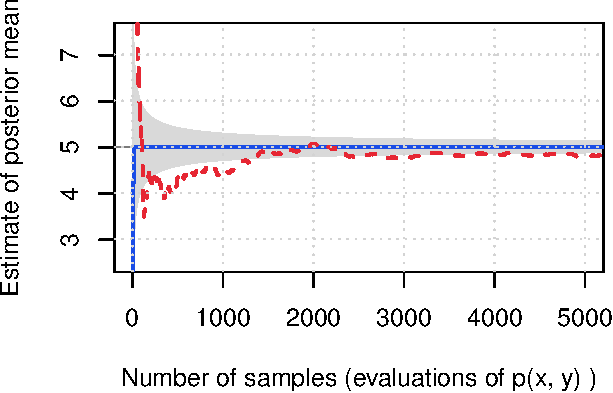
\includegraphics[width=0.8\textwidth,height=0.5\textwidth]{chapter_stochastic_variational_optimization/figures/posterior_mean_estimates_all.pdf}
    \caption{figure}{SVO can converge quickly to a univariate
      non-conjugate posterior $p(x | y)$.  Solid blue: the estimated
      mean of a variational posterior against the number of samples
      (and evaluations of the joint) using second-order SVO.  Dashed
      red: estimated mean of the posterior using a Metropolis-Hastings
      sampler. Shaded: 95\% confidence intervals of the mean
      estimate from an oracle sampler.}
  \label{figure:univariate_comparison}
}

\newcommand{\changepointdata}[0]{
  \center
  \begin{tabular}{|c|c|c|}
    \hline
    \multicolumn{3}{|c|}{Switching Kalman filter (well log data)} \\ 
    \hline
    \textbf{Metric} & \textbf{SVO} &  \textbf{Gibbs} \\
    \hline
    \textbf{\footnotesize Heldout MSE} & \footnotesize 3.6e6 & 3.5e6 \\
    \hline
    \textbf{\footnotesize Time} & 92 sec. & 104 sec. \\
    \hline
    \textbf{\small ``True'' MSE} & 2.2e6 & 2.4e6 \\
%    \textbf{\small Gibbs 50K} &  &  \\
    \hline
  \end{tabular}
}

\newcommand{\changepointplot}[0]{
  \center
  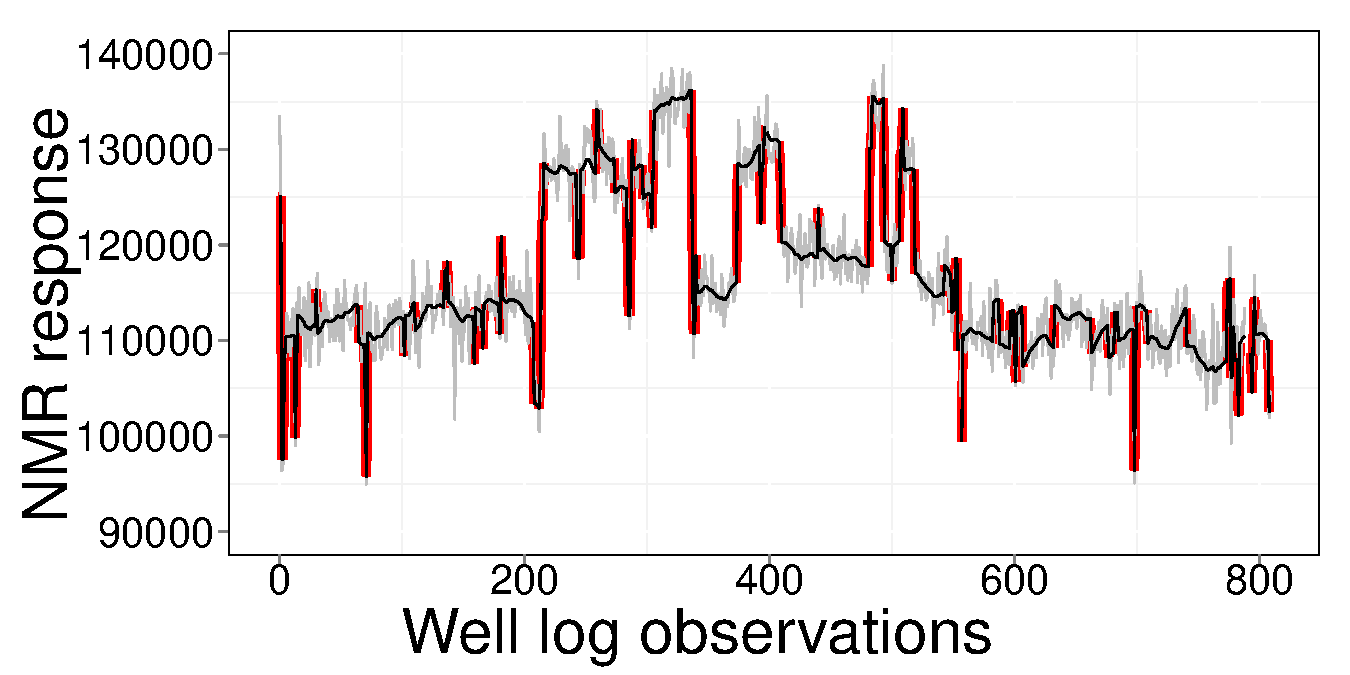
\includegraphics[width=0.8\textwidth,height=0.465\textwidth]{chapter_stochastic_variational_optimization/figures/changepoint_analysis_example_time_series.pdf}
  \vspace{5pt}
  \caption{Well-log data (grey) fit with a variational switching
    Kalman filter. The inferred means $\bar \mu_{t}$ of the filter are shown in black.  Each timestamp also has an associated variational change point $\bar c_t$ which indicates the probability that the filter is making a large transition.  Transitions at change points with mean $\bar c_t > \frac{1}{2}$ are marked in red.}
  \label{figure:switching_kalman_filter}
}

\newcommand{\irtdata}[0]{
  \center
  \begin{tabular}{|c|c|c|c|}
    \hline
    \multicolumn{4}{|c|}{\normalsize Probit Item Response Theory} \\
    \hline
    \textbf{Metric} & \textbf{SVO} & \textbf{Variational} & \textbf{Gibbs} \\
    \hline
    \textbf{\footnotesize Heldout LL} & \footnotesize -0.181 & -0.214 & -0.214 \\
    \hline
    \textbf{\footnotesize Time} & 27 sec. & 5 sec. & 122 sec. \\
    \hline
%    \textbf{\small MSE,} & 0.057 & --- & --- \\
%    \textbf{\small variational} &  &  & \\
%    \hline
    \textbf{\small ``True'' MSE} & 0.048 & 0.031 & 0.001 \\
    \hline
  \end{tabular}
}

\begin{figure*}
  \center
  \begin{tabular}{c}
    \begin{minipage}{5.7in}{
        \center \irtdata }
    \end{minipage}
    \\
    \begin{minipage}{5.7in}{
        \center \changepointdata }
    \end{minipage}
  \end{tabular}
  \caption{Experimental results comparing SVO and MCMC estimates. We
    show lawmaker posteriors in the probit IRT model (left) and
    observation means from a change point model (right).  In each
    table we illustrate runtime, log-likelihood (LL) or mean-squared
    error (MSE) on heldout observations. We also estimate MSE against
    the ``True'' posterior means, estimated using long Gibbs runs
    (500K and 50K samples for left and right respectively).  }
  \label{figure:changepoint_results}
  \label{figure:irt_results}
\end{figure*}

\begin{figure*}
  \begin{tabular}{c}
    \begin{minipage}{6in}{
        \center \univariatefigure }
    \end{minipage}
    \\
    \begin{minipage}{6in}{
        \center \changepointplot }
    \end{minipage}
  \end{tabular}
\end{figure*}

% dmb: above, these two tables look funny together in the same
% figure.  let's put them in separate figures and call them
% "Figure"---we don't need to differentiate in such a short paper
% between table and figure.  also, see my note below.  i'm not sure weuuuu
% need MSE variational.  and maybe we can call MSE Gibbs 500K "True
% MSE" (or something so it's on one line.  Also Log L'hood is not
% clearly held out Log L'hood or predictive log l'hood.


\textbf{Oracle sample} The above comparison with a specific MCMC
sampling method depends on our choice of MCMC algorithm and parameters
such as the proposal distribution.  Therefore we also compare with an
oracle sampler, which provides error bounds on the best possible $iid$
sampling algorithm (most standard MCMC algorithms produce samples
which, when thinned, are treated as \emph{iid}).  An oracle sampler is
able to draw \emph{iid} samples from p(x, y) to estimate the mean.
For each sample size $M$, we explicitly calculate the 95\% standard
error confidence intervals of an estimated mean from $M$ samples.  We
plot these error bars around the true mean in
Figure~\ref{figure:univariate_comparison}.  Even with a perfect
sampler, an estimate of the mean takes much longer to converge than
univariate SVO.

\subsection{Probit regression and ideal points}
\label{section:probit_regression}
We next studied SVO for approximating a complex posterior in a large
high-dimensional model.

We fit a matrix of U.S. lawmakers' votes using Item Response Theory
(IRT), a class of models frequently used in political science
\cite{poole:1991,martin:2002,albert:1992}.  IRT is used to position
each lawmaker $l$ in a latent space with positions $x_l \in
\mathbb{R}$; these positions are often studied by political scientists
to understand the lawmakers' political preferences.  Lawmakers'
positions interact with latent bill variables $a_d, b_d \in
\mathbb{R}$; all latent variables take a standard normal prior.  The
probability of lawmaker $l$ voting ``Yes'' on bill $d$ is then given
by $p(v_{ld} = \mbox{Yes}) = \mbox{probit}(x_l a_d + b_d)$
\cite{clinton:2004}.

\textbf{Experiments.}  Political methodologists usually implement
these models with MCMC methods \cite{albert:1992} (a variational
implementation was introduced in \cite{gerrish:2011}, although that
used the logistic response). We fit these models with MCMC,
traditional variational Bayes, and SVO.  We chose fully-factorized
Gaussian posterior distributions.
% \[
% p(x_1, \ldots, x_L, a_1, b_1, \ldots, a_D, b_D) = \prod_L \prod_D \mathcal{N}(x_\bar 
% \]

We can use an auxiliary random variable to yield a fast Gibbs sampler
and a variational algorithm \cite{armagan:2011} (this is not possible
with a logistic response).  We fit the posterior with these algorithms
as well as with second-order SVO.

\textbf{Results.} We estimated the means of these random variables for
68 Senate bills, 95 senators, and 5,145 votes during the years
2009-2010 (this was 219 dimensions).  We fit these models and compared
the estimated means $\bm \bar x, \bm \bar a, \bm \bar b$ of ideal
points and bill variables; we summarize the results in
\myfig{irt_results}.  MCMC was the slowest, while traditional
variational inference was the fastest.  The latter is not surprising
because variational Bayes uses coordinate ascent, while SVO uses
slower Newton-Raphson updates on coordinates.  (Further, the
variational algorithm takes advantage of the derivatives of the ELBO,
which we do not need to derive for SVO.)

We estimated the ``true'' posterior mean using 500,000 MCMC samples
and found that the means estimated with both variational Bayes and
MCMC samplers were closer to the ``true'' mean than means estimated
with SVO.  However, we also assessed the posteriors by their
predictive distribution, using six-fold cross validation to measure
log-likelihood on held-out votes.  SVO formed much better predictions
than the other two algorithms. (The difference between SVO and the
variational Bayes estimates is explained by the auxiliary variable.)

% dmb: above, i'm not sure its clear what the difference is between
% Gibbs 500K and Gibbs.  And, do we need MSE, variational in the
% table?  we don't describe it and it's also not clear what it means.
% (i can infer, but then why isn't their a number for Gibbs?)
% smg: I removed MSE, variational.  I can clarify the difference
% between gibbs and gibbs500k.

\subsection{Switching Kalman filter}
\label{section:switching_kalman_filter}
We next illustrate this method in the task of identifying change
points---positions of large changes---in a time-series dataset.  To
this end, we assume a series of real-valued observations $y_{1:T}$
arising from underlying means $\mu_{1:T}$.  These means transition
with low variance but occasionally make a large transition.  These changes
are characterized by random switch variates, $c_t \in \{ 0, 1 \}$,
which may indicate a large transition ($c_t=1$) with low probability. This
distribution---a switching Kalman filter \cite{murphy:1998}---has the
density
\begin{align}
  \vspace{-14pt}
  p(c_{1:T}, \mu_{1:T}, y_{1:T}) = p(\mu_1) p(\mu_T) \textstyle
  \prod_{t=2}^T p(c_t) p(y_t | \mu_t) p(\mu_t | \mu_{t-1}),
\end{align}
with Gaussian observation density $p(y_t | \mu_{t-1})$ and Gaussian
transition probabilities (with variance depending on $c_t$).  $p(c_i)$
is the probability of a change point, with $p(c_i) = 0.001$. While the
conditional distributions are conjugate (enabling fast Gibbs
samplers), there is no analytical solution to describe the posterior
distribution, so variational approximations are sometimes used
\cite{ghahramani:1996,murphy:1998}.  (The derivation of the
variational inference algorithm in \cite{ghahramani:1996} was 2.5
pages.)

\textbf{Experiments.} We implemented this model using both a Gibbs
sampler and SVO. We used the fully-factorized posterior $\prod_T
q(c_t | \bar c_t) q(\mu_t | \bar \mu_t)$ of Bernoulli and Gaussian variational
distributions. We fit this model to a set of 809 measurements taken
during the drilling of a well using nuclear magnetic resonance
(NMR). The well log data were ``used to interpret the geophysical
structure of the rock surrounding the well'' \cite{adams:2007} and
have been studied previously using change point models
\cite{ruanaidh:1996,adams:2007}. We illustrate these data (along with
SVO posterior means) in \myfig{switching_kalman_filter}. We fixed the
variances and $\pi$ by a-priori estimation for the well data before
fitting any models.

\textbf{Results.} We summarize these results in
\myfig{changepoint_results} and in \myfig{switching_kalman_filter}.
We first observe that SVO takes nearly as long to converge as a
1500-sample (after 500 burn-in) Gibbs run.  Why is this? In this
specific case, the Gibbs sampler is very high-quality, drawing
``oracle'' examples with high probability once it has burned in. SVO's
time performance suffers because it wastes effort updating variables
that are highly dependent.

We compared these posterior estimates with posterior means from a
49,500-sample Gibbs run, which we treat as ground truth.  In contrast
to the IRT experiment, the SVO fit estimated better posterior means
than the 1500-sample Gibbs estimate, and SVO estimated a predictive
distribution which is no better than the Gibbs estimate. This is
surprising but may be because the Gibbs sampler had not
converged. Although the estimated means $\mu_t$ of these distributions
were similar, the variational distribution discovered nearly three
times as many active change points (i.e., $\bar c_t > 0.5$) as either Gibbs
posteriors, illustrating the inherent bias in variational methods.

%\begin{table}
%  \begin{tabular}{|c|c|c|}
%    \hline
    %\multicolumn{3}
%    \textbf{Model} & \textbf{MSE 50k} & \textbf{} %\\
%    \hline
%  \end{tabular}
%\end{table}

\subsection{Alternative variational distributions: Laplace variational posterior}
\label{section:complicated_posteriors}
We have discussed variational Gaussian and multinomial posteriors,
which are both commonly used in variational inference.  But SVO opens
the door to many kinds of variational distributions, as all we require
is to sample from them and compute the gradient of their logs.  In \S
A.4, we report a study fitting $L_1$-regularized logistic regression
with a multivariate Laplace variational posterior on two standard
datasets.  This factorized Laplace posterior had the density $q_{\bm
  \mu, \kappa}( \bm \beta ) = \propto \exp( - \exp(\kappa) \sum_I |
\beta_i - \mu_i | )$, with free variational parameters $\mu_1, \ldots,
\mu_d$ and $\kappa$.  This leads to a ``fat-tailed'' posterior which
estimates posterior means which are closer to the prior mean.  Importantly,
these posterior distributions yielded higher held-out log-likelihood
performance This and similar alternative posteriors are interesting
avenues for future work.

% dmb: above, can you give the punch line of the laplace experiment?
% you may even have room for a small table.

% We applied this variational posterior to several datasets from the UCI
% repository: \verb!ionosphere!, \verb!car!, and \verb!statlog!.  Each
% of these datasets contains a binary classification problem using tens
% of covariates and hundreds or thousands of training examples (for
% \verb!statlog!, we predicted the \emph{sky} label).  We fit the
% regression problem above to each of these datasets with both a
% variational Gaussian posterior and a variational Laplace posterior.
% In each case, we fixed $\lambda = 50$.

% Figure~\ref{figure:gaussian_vs_laplace} shows coefficients fit from
% both of these models.  The variational posterior, as expected, tends
% to push its coefficients toward zero.  The two posteriors performed
% nearly equally: the Gaussian posterior was slightly better in the
% \verb!car! dataset, while the two were indistinguishable in the
% \verb!ionosphere! and \verb!statlog! datasets.
% %% \begin{figure*}
% %%   \begin{tabular}{ccc}
% %%   \includegraphics[width=0.3\textwidth]{figs/car_gaussian_vs_laplace.pdf} &
% %%   \includegraphics[width=0.3\textwidth]{figs/ionosphere_gaussian_vs_laplace.pdf} &
% %%   \includegraphics[width=0.3\textwidth]{figs/segment_gaussian_vs_laplace.pdf} \\
% %%   (a) & (b) & (c) \\
% %%   \end{tabular}
% %%   \caption{Comparison of coefficient values using different
% %%     variational posteriors in $L_1$-regularized logistic regression.
% %%     Solid points are coefficient values fit with a Laplace posterior,
% %%     and hollow points are values fit with a Gaussian posterior. (a),
% %%     (b), and (c) are the car, ionosphere, and segment datasets, respectively.}
% %%   \label{figure:gaussian_vs_laplace}
% %% \end{figure*}
% The reader may note that the \verb!statlog! Laplace coefficients shown
% in Figure~\ref{figure:gaussian_vs_laplace} do not always agree with
% the Gaussian coefficients.  Upon inspection, we found that the
% variational Laplace solutions were fairly uncorrelated in successive
% runs (e.g., $\rho=0.34, 0.25, 0.40$), while the Gaussian posteriors
% were much more correlated ($\rho=0.93,0.90,0.88$).  Despite this, all
% solutions correctly classified over 98\% of items correctly. As
% variational inference solves an optimization problem, the Laplace
% posterior appears more likely to converge to different modes on
% subsequent runs.

%% \subsection{Variational stochastic optimization}
%% In this section, I will provide a comparison with Carbonetto et al.
%% \cite{carbonetto:2009}.

% \begin{figure}
%   \includegraphics[width=0.25\textwidth]{figs/gaussians_mean.pdf}
%   \includegraphics[width=0.25\textwidth]{figs/gaussian_approximation.pdf}  \\
%   \caption{Left: convergence of the variational mean (green) to a true
%     Gaussian distribution with mean 5, compared with an MCMC sampler
%     (red) with different burn-in times (dotted, solid). The horizontal
%     line is a Metropolis estimate of the mean after 50,000 iterations.  Right: an
%     illustration of the variational approximation of the true density
%     (the variational distribution and true density are the same line)}
%   \label{figure:convergence1}
% \end{figure}

% \begin{figure}
%   \includegraphics[width=0.25\textwidth]{figs/mixture_gaussians_mean.pdf}
% %  \includegraphics[width=0.25\textwidth]{figs/mixture_gaussians_variance.pdf} \\
%   \includegraphics[width=0.25\textwidth]{figs/gaussian_mixture_approximation.pdf} \\
%   \caption{Left: convergence of the variational mean (green) to a
%     mixture-of-Gaussians distribution, compared with an MCMC
%     sampler (red) with different burn-in times (dotted, solid).  The
%     horizontal line is a Metropolis estimate of the mean after 50,000
%     iterations.  Right: an illustration of the variational
%     approximation of the true density.}
%   \label{figure:convergence2}
% \end{figure}

% \begin{figure}
%   \includegraphics[width=0.25\textwidth]{figs/laplace_mean.pdf}
% %  \includegraphics[width=0.25\textwidth]{figs/laplace_variance.pdf}
%   \includegraphics[width=0.25\textwidth]{figs/laplace_approximation.pdf} \\
%   \caption{Left: convergence of the variational mean to the density $p
%     \propto \exp(\frac{(x-5)^2}{8} - \frac{1}{2} \log (2 \pi) -
%     \frac{1}{2} \log(4)) \times \exp(-|2 x|)$. Variational
%     approximation is in green, along with an MCMC approximations (red)
%     with different burn-in times (dotted, solid).  The horizontal line
%     is a Metropolis estimate of the mean after 50,000 iterations.
%     Right: an illustration of the variational approximation of the
%     true density.}
%   \label{figure:convergence3}
% \end{figure}

%% \subsection{Variational linear regression}

%% I haven't had time to implement this section of the experiments yet.
%% We'll see whether it's necessary.

% We demonstrate variational linear regression, y = beta' x + e, on a
% ~20-dimensional dataset, using our method to estimate E var(beta) and
% E var(y | x, beta). We demonstrate that we get (1) better predictive
% performance than variational linear regression and MCMC, which is due
% to (2) better estimation of E [ 1 / var(y | x, beta) ].  We plot the
% latter for our method, MCMC (to estimate "true" precision), and
% standard variational linear regression.  Variational linear regression
% took x seconds, our method took xx seconds, and MCMC took xx minutes.
% Discussion of why this happens.

%%% Local Variables: 
%%% mode: latex
%%% TeX-master: "nips2012"
%%% End: 

\section{Discussion}

We described stochastic variational optimization, a generic method for
variational inference that does not require taking gradients of the
evidence lower bound.  SVO uses stochastic optimization, taking
advantage of second-order updates and quasi-Monte Carlo sampling to
improve this optimization.  The main benefit of SVO is that it is
independent of the functional form of $p(x, y)$.  With a cache of
sampling methods and gradients of variational distributions, we can us
SVO to rapidly build and fit many kinds of models.  We demonstrated
that SVO provides a good fit to the variational objective, often
forming superior predictive distributions to competing algorithms.

% % We demonstraexperiments and Carbonetto \cite{carbonetto:2009} demonstrate the range of applications on which  this method with LDA
% % \cite{blei:2003}; as we will demonstrate in the experiments, this
% % method can be used for a wider variety of statistical models, with
% % clear benefits over both MCMC and traditional variational inference

% %%  The motivation for
% %% black-box variational methods is similar to the motivation for
% %% Expectation Propagation \cite{minka:2001}: speed and simplicity.

% %% Another benefit of SVO is that can be fast: each sample
% %% provides specific information about the gradient of the objective,
% %% turning the problem into a gradient ascent problem.  MCMC methods
% %% differ in that they must search through the sample space and may
% %% discard many samples.  Although these discarded samples provide useful
% %% information indirectly, a poorly chosen proposal distribution may mean
% %% most of the samples are rejected; even when they are used, they
% %% typically are no better than \emph{iid} samples.

% % SVO does not require $p(x, y)$ to be conjugate to the variational
% % posterior. This sets it apart from traditional variational methods, in
% % which the variational posterior must be conjugate to the joint
% % likelihood for symbolic manipulation to work out, without resorting to
% % approximations.


% %%   When this is not
% %% the case, further assumptions typically must be made to make inference
% %% tractable.

% %% A final benefit of SVO is that it has an explicit, commonly used
% %% objective function.
% %% %% Then the objective (Equation~\ref{equation:objective}) measures the
% %% %% goodness-of-fit and has an upper bound of zero. 
% %% Progress and convergence of the algorithm can be monitored with this
% %% objective even when the posterior is unnormalized.
% %  In MCMC, there is no explicit objective.

% % \paragraph{Limitations of SVO}
% Because SVO optimizes the variational objective, it suffers from all
% of the shortcomings of variational inference.  One of these
% limitations is that variational methods can get stuck in local
% optima. In addition, the variational estimate may be biased.

% Our algorithm is not guaranteed to converge, e.g. when the objective
% has positive curvature; this is a problem with Newton-Raphson
% optimization in general. Another problem we have observed is that
% posteriors with large variances can lead to poor estimates of a mean.

% %\paragraph{Areas for future work}
% %
% These limitations suggest further areas for improvement.  One of these
% is exploration of flexible variational families which can mitigate
% bias.  Problematic curvature might be solved with a stochastic version
% of line search. Finally, one of the most promising areas for future
% work is development of black-box libraries for probabilistic
% inference.  \vspace{-2pt}

%% The authors also found the following rules-of-thumbs to be helpful:
%% \begin{itemize}
%% % \item Begin with first-order stochastic updates. Move to second-order
%% %   updates once the first-order updates have reached a mode.
%% % \item The first-order learning rate $\eta_\sigma$ can be set so that
%% %   the variance neither doubles nor halves with a typical update.  The
%% %   rate can be decreased whenever an update exceeds this value.
%% % \item The first-order learning rate $\eta_\mu$ can be set so that the
%% %   unweighted update for $\mu$ does not move more than five standard
%% %   deviations.  The rate can be decreased whenever an update exceeds
%% %   this value.
%% \item Avoid first-order updates whenever possible.  While these
%%   updates work well when the learning rate is well-chosen, a
%%   poorly-chosen learning rate may make the model converge more slowly.
%% \item Use enough samples for second-order updates.  Fifty to a few
%%   hundred is a good rule-of-thumb.
%% \item During second-order updates, use a convex combination of the
%%   current parameter and the proposed parameter.  Although the update
%%   should put the parameters close to the correct position, and the
%%   Taylor approximation can be estimated arbitrarily well, the
%%   approximation remains only an approximation.  This also smooths out
%%   noise from sampling.
%% \end{itemize}


%%% Local Variables: 
%%% mode: latex
%%% TeX-master: "nips2012"
%%% End: 
